%----------------------------------------------------------------
%
%  File    :  survey-examples.tex
%
%  Author  :  Keith Andrews, IICM, TU Graz, Austria
% 
%  Created :  18 May 2012
% 
%  Changed :  18 May 2012
% 
%----------------------------------------------------------------

\chapter{Selected Examples of Doing Things with \LaTeXe\
(and Test of Extremely
Long Chapter Titles to See How They Work Or Not)
}

\label{chap:SelectedExamples}


This chapter contains some examples of typical \LaTeXe\
usage.




\section{First Selected Example}

An example of using a table can be seen in Table~\ref{tabBestPubs}.

\begin{table}[tp]
\centering
\begin{tabular}{|llrp{10cm}|}
\hline
Name & Type & Rating & Description \\
\hline
The Office &
English &
***** &
The best pub in Graz. Hidden in the narrow streets
of the old town. A wonderful hideout for ex-pats.
A pint of Guinness for only \euro 3.90.
\\
\hline
Flann O'Brien &
Irish &
**** &
In the centre of town and easy to find for
marauding tourists.
\\
\hline
O'Carolans &
Irish &
**** &
In the centre of town in a small side street next to Flann's.
Small, cosy Irish pub.
\\
\hline
O'Riginal &
pseudo Irish &
 &
Austrian dive pretending to be an Irish pub.
Definitely not my cup of tea.
\\
\hline
\end{tabular}

\caption[Best Pubs in Graz]
{
The best pubs in Graz.
}
\label{tabBestPubs}
\end{table}





\section{Second Selected Example}

This example shows how to inculde vector graphics in the form of PDF
files. It also shows how to use subfigures within a figure.


\begin{figure}[tp]
\centering
\subfloat[
A object has been composed to represent an
abstract version of the clock tower in Graz.
Here, the object is in its initial state.
]
{
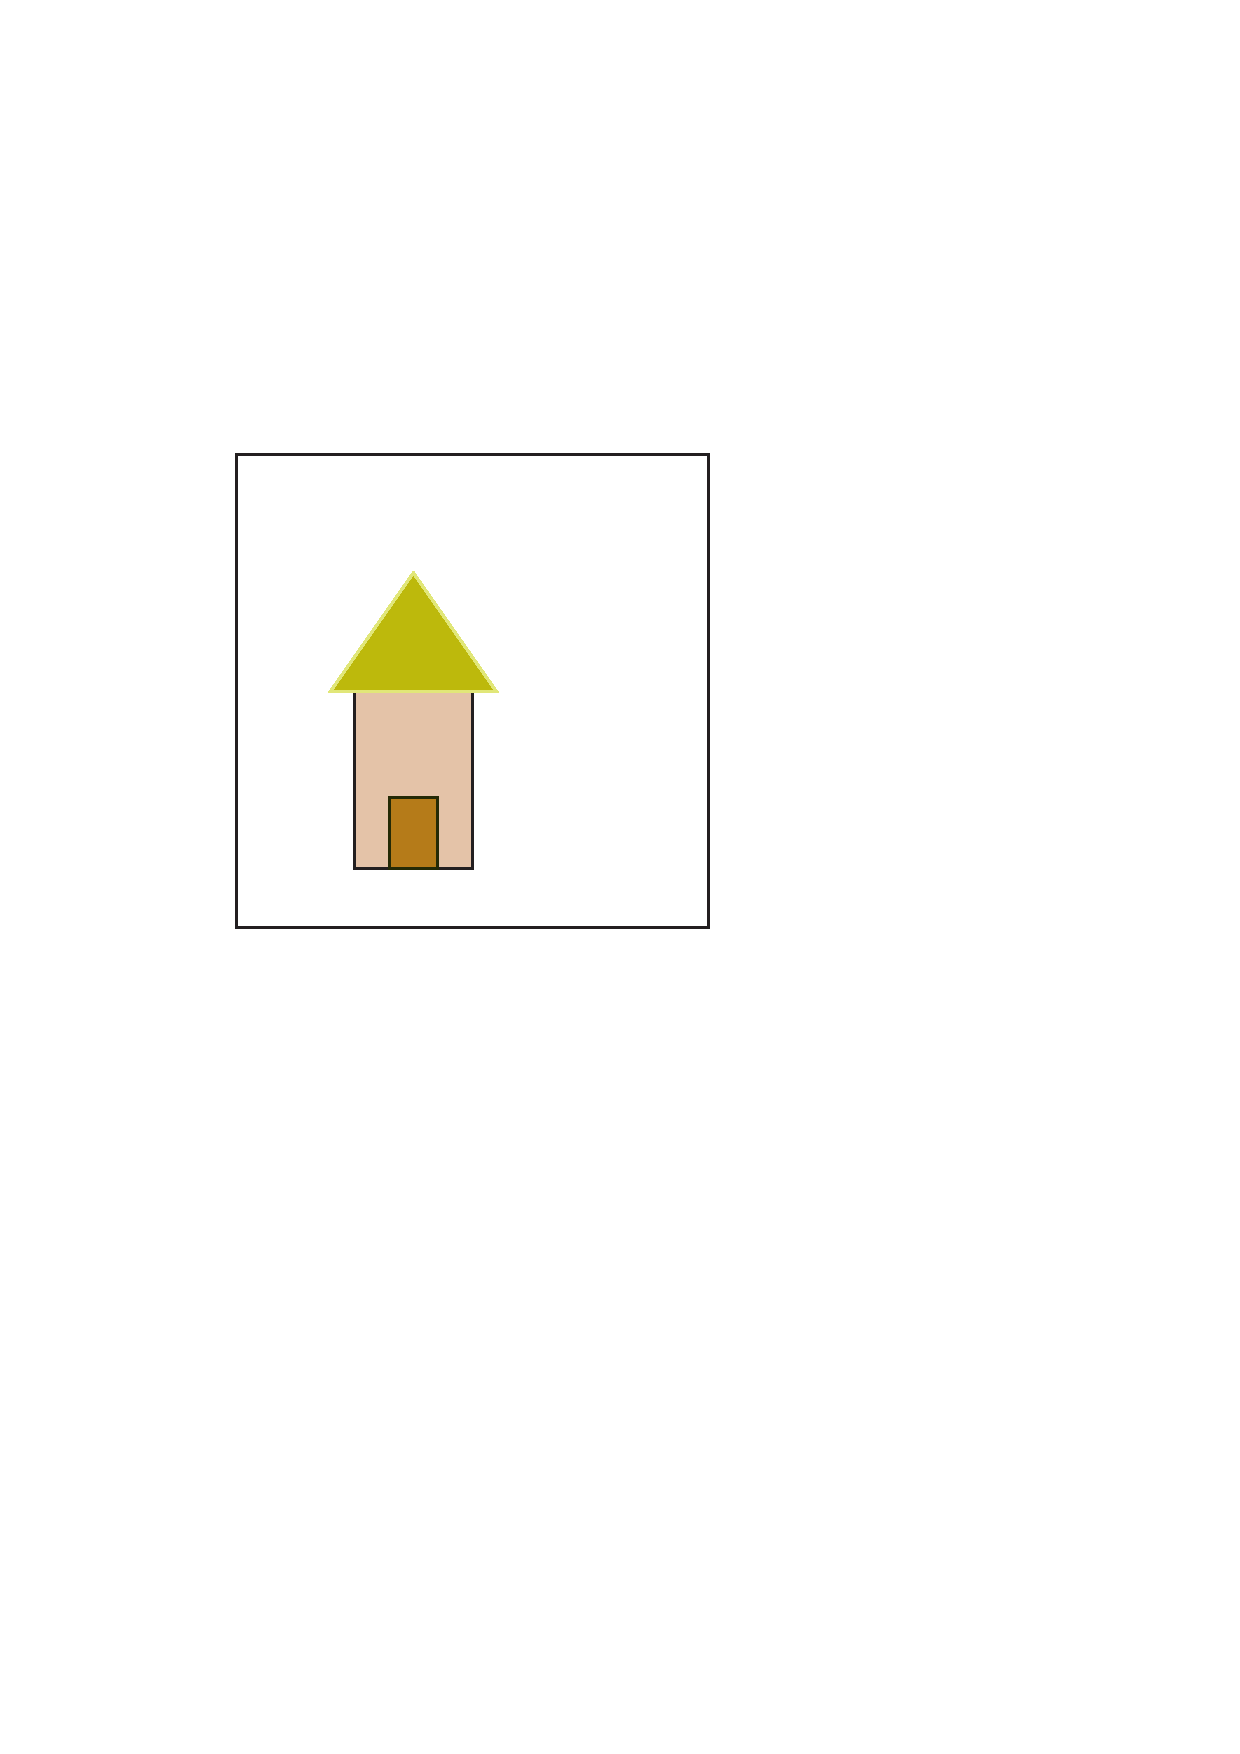
\includegraphics[width=0.45\hsize]{diagrams/multi1}
\label{figTower1}
}
\hfill
\subfloat[
The object has been scaled and rotated, and now resembles
a leaning tower.
]
{
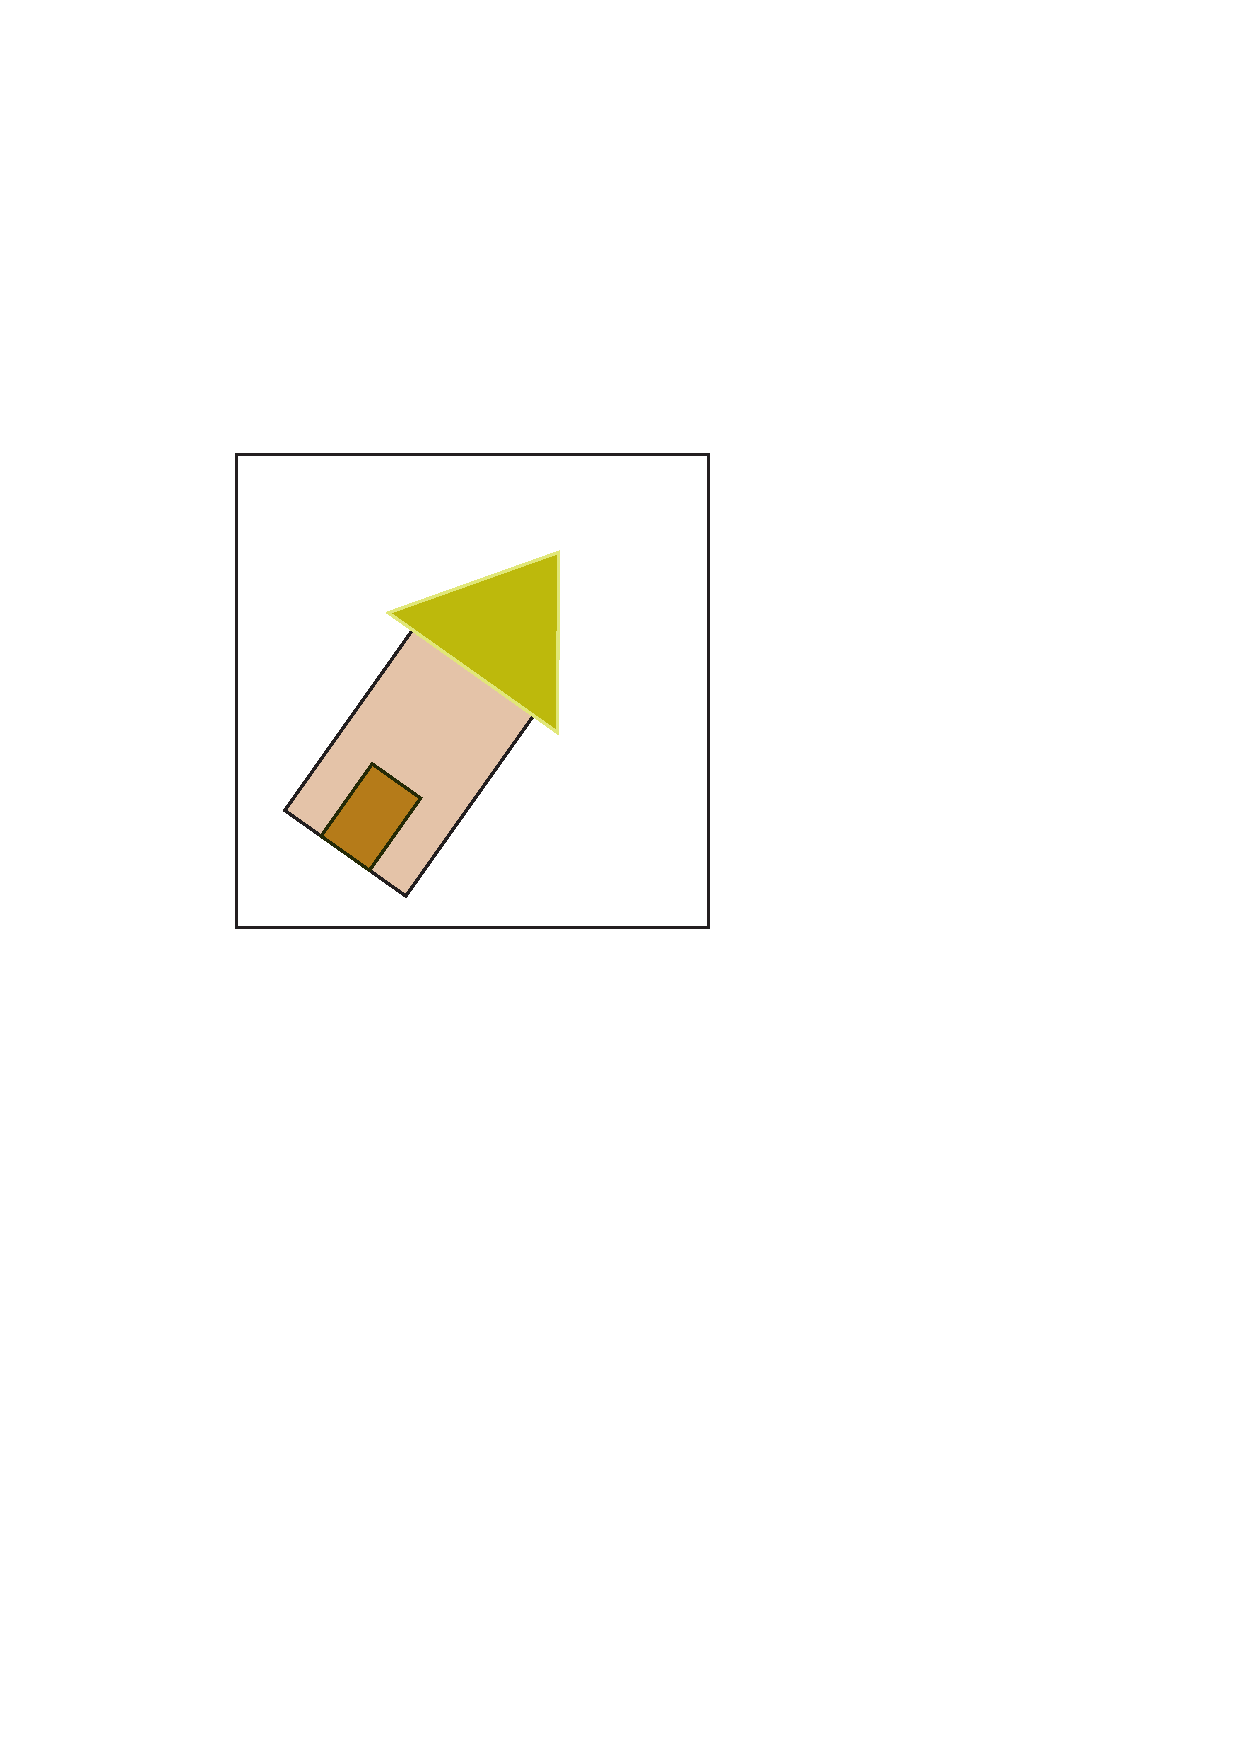
\includegraphics[width=0.45\hsize]{diagrams/multi2}
\label{figTower2}
}

\caption[Abstract Clock Towers]
{
The leaning tower of Graz. An abstract model of the clock
tower in Graz leaning over time. \subref{figTower1} shows
the initial state. \subref{figTower2} shows the final state.
}
\label{figWholeFig}
\end{figure}


An example of using the \vname{subfig} package can be seen in
Figure~\ref{figWholeFig}. Figure~\ref{figTower1} shows the polygons
before transformation, while Figure~\ref{figTower2} shows them
afterwards.




\section{Third Selected Example}


This example shows how to include a screen shot (or other raster
graphic) into a \LaTeXe\ figure.

\begin{figure}[tp]
\centering
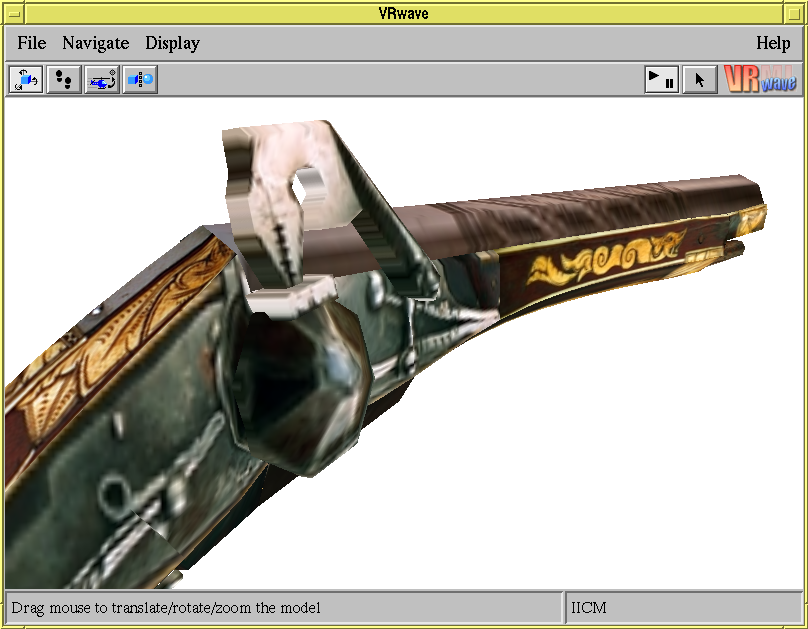
\includegraphics[keepaspectratio,width=\hsize]{images/pist}

\caption[VRwave in Flip Mode]
{%
VRwave in Flip mode displaying a textured model of a cavalry pistol
from the world-renowned Zeughaus (armoury) in Graz.
\imgcredit{Image extracted from \citet[page 81]{Andrews-VRwave}
under the terms of the ACM copyright. \copyrightACM}
}
\label{fig:Pistol}
\end{figure}


An example of how to correctly cite the source when using an image
from someone else. In their 1998 paper, \citet{Andrews-VRwave} discuss
the VRwave VRML browser. Figure~\ref{fig:Pistol} shows a VRML model of
a cavalry pistol from the Armoury in Graz displayed in the VRwave VRML
browser.





\section{Fourth Selected Example}

You can use many (but not all) of the thousands of characters
available in the UTF-8 \citep{Wikipedia-UTF8,Unicode-Charts} character
encoding. For example, the German umlauts (äüö), the German sharp s
(ß), or the yen symbol (¥).

You can also try some of the \approxsym 100 symbols available
in the \vname{textcomp} package, such as the yen symbol (\textyen) and
a circled letter A (\textcircled{A}).

Use the \vname{vname}, \vname{cname}, and \vname{fname} macros to
define the style for variable names, class names, and file names. You
can also define your own macros. The is a very long file name
\fname{/usr/data/keith/travel/austria/vienna.txt} to see how they are
broken at a line end. A typical class name is
\cname{HVSInformationPyramidsInputFactory}.






\section{Fifth Selected Example}

Sometimes, a macro (new command definition) can be useful to define
the contents of table cells, particularly if these contain images. For
example, Table~\ref{tab:WinIconicLang} uses the macro called
\vname{iibox}, which takes a single parameter, the name of
the particular image.



\begin{table}[tp]

\newcommand{\iibox}[1]{\parbox[c][1cm][c]{1cm}{%
\includegraphics[scale=0.6]{./images/icons/#1}
}}

\begin{center}
\begin{tabular}[t]{|p{7cm}c|}
\hline
\multicolumn{2}{|l|}{\sffamily \bfseries Elementary Symbols}            \\
Document                            & \iibox{win-il-gen-doc}            \\
Assistant                           & \iibox{win-il-gen-ass}            \\
Template                            & \iibox{win-il-gen-tmpl}           \\
\hline
\multicolumn{2}{|l|}{\sffamily \bfseries Document Types}                \\
Text document                       & \iibox{win-il-text-doc}           \\
Spreadsheet document                & \iibox{win-il-spreadsheet-doc}    \\
Presentation document               & \iibox{win-il-presentation-doc}   \\
Database document                   & \iibox{win-il-database-doc}       \\
\hline
\multicolumn{2}{|l|}{\sffamily \bfseries Applications}                  \\
Word                                & \iibox{win-il-word-appl}          \\
Excel                               & \iibox{win-il-xls-appl}           \\
Powerpoint                          & \iibox{win-il-ppt-appl}           \\
Access                              & \iibox{win-il-mdb-appl}           \\
\hline
\multicolumn{2}{|l|}{\sffamily \bfseries Generated Icons}               \\
Word text document                  & \iibox{win-il-word-doc}           \\
Excel spreadsheet document          & \iibox{win-il-xls-doc}            \\
Powerpoint presentation document    & \iibox{win-il-ppt-doc}            \\
Access database document            & \iibox{win-il-mdb-doc}            \\[2ex]
%
Word template                       & \iibox{win-il-word-tmpl}          \\
Powerpoint template                 & \iibox{win-il-ppt-tmpl}           \\
Access template                     & \iibox{win-il-mdb-tmpl}           \\[2ex]
%
Word template assistant             & \iibox{win-il-word-ass}           \\
Powerpoint template assistant       & \iibox{win-il-ppt-ass}            \\
Access template assistant           & \iibox{win-il-mdb-ass}            \\[2ex]
%
\hline
\end{tabular}
\end{center}

\caption[Iconic language for Windows NT 4.0 documents]
{
Iconic language for Windows NT 4.0 documents.
}
\label{tab:WinIconicLang}
\end{table}




\section{Textual Citations}

\citet{DataAnalysisChallenges} define visual analytics as:
\begin{quotation}
``iterative process that involves collecting information, data
  preprocessing, knowledge representation, interaction, and decision
  making''.
\end{quotation}


\citet[Chapter~7]{InteractiveDataVisualisation} categorise
visualisation techniques for multi-variate data according to the
graphical primitive used in the rendering: points, lines, and regions.


